\documentclass[usenames, dvipsnames, compress]{beamer}
\usepackage[utf8]{inputenc}
\usetheme{metropolis}
\usepackage{graphicx}
\usepackage{booktabs}
\usepackage{amsthm}
\usepackage[T1]{fontenc}
\usefonttheme{professionalfonts}
\usepackage{xcolor}
\usepackage{color}

\usepackage{listings}


\usepackage{minted}
\usemintedstyle{manni}
\newminted{python}{fontsize=\footnotesize}


% Define colors

\definecolor{mygray}{rgb}{0.5,0.5,0.5}
\definecolor{eafitcolor}{HTML}{010068}
\definecolor{textcolor}{HTML}{0400E6}
\definecolor{blockcolor}{HTML}{0300CC}
\definecolor{blockbodycolor}{HTML}{E6E6FF}
% Settings
\setbeamercolor{background canvas}{bg=White}
\setbeamertemplate{frame footer}{Universidad EAFIT}
\setbeamercolor{example text}{fg = White}
\setbeamercolor{palette primary}{fg=White, bg=eafitcolor}
\setbeamercolor{progress bar}{fg=Blue,bg=Periwinkle}
\setbeamercolor{alerted text}{fg=eafitcolor}
\setbeamercolor{frametitle}{bg=eafitcolor, fg=White}
\setbeamertemplate{section in toc}[sections numbered]
\setbeamercolor{block title}{use=structure,fg=white,bg=blockcolor}
\setbeamercolor{block body}{use=structure,bg=blockbodycolor}


%\setbeamertemplate{subsection in toc}[subsections numbered]


%\logo{
\includegraphics[height=1cm]{logo.png}}
\title[Octave y Python]{Introducción a la Programación}



\author{Anderson Daniel Grajales Alzate}
\institute[Universidad EAFIT]
{Análisis Numérico / Procesos Numéricos \\ % Your institution for the title page
	\medskip
	\textit{agrajal7@eafit.edu.co} % Your email address
	
}

\date{Febrero 25 de 2019}
\newtheorem{defa}{Definición}
\newtheorem{dnote}{Nota}
\newtheorem{pyth}{Python}
\newtheorem{octa}{Octave}



\begin{document}
	\begin{frame}
		\titlepage % Print the title page as the first slide
	\end{frame}
	\begin{frame}[allowframebreaks]{Contenidos}
		\tableofcontents
	\end{frame}
	\section{Algoritmos}
	\subsection{Definición}
	\begin{frame}{Algoritmo}
		\begin{defa}
			Secuencia cronológica y ordenada de pasos que llevan a la solución de un problema o a la ejecución de una tarea o actividad.
		\end{defa}
	\end{frame}
	\subsection{Características}
	\begin{frame}{Características}
		\begin{itemize}[<+- | alert@ +>]
			\item \textbf{Finito: } Debe terminar después de un número finito de pasos.
			\item \textbf{Definido: } Cada paso debe estar bien precisado y no debe haber ambigüedad en ninguno de éstos.
			\item \textbf{Entrada: } Debe tener cero o más entradas.
			\item \textbf{Salida: } Debe tener al menos una salida.
			\item \textbf{Efectivo}: Cada operación debe ser lo suficientemente básica, de tal forma que la ejecución de la misma termine en un tiempo finito.
		\end{itemize}
	\end{frame}
	\section{Pseudocódigo}
	\subsection{Definición}
		\begin{frame}{Pseudocódigo}
			\begin{itemize}[<+- | alert@+>]
				\item Serie de pasos o procedimientos que permiten alcanzar un resultado o resolver un problema.
				\item Describe un algoritmo utilizando una mezcla de frases en lenguaje común, instrucciones de programación y palabras clave que definen las estructuras básicas.
				\item No necesariamente siempre es estándar en cada algoritmo que se escribe.
				\item Uso lenguaje natural para expresar el funcionamiento de diferentes procedimientos.
			\end{itemize}
		\end{frame}
	\subsection{Partes}
	\begin{frame}{Entrada}
		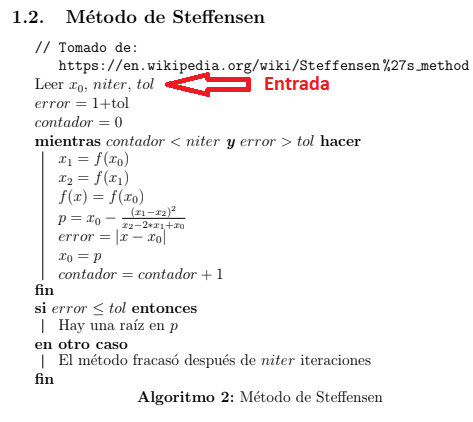
\includegraphics[height=230pt]{images/entrada.png}
	\end{frame}
	\begin{frame}{Procedimiento}
		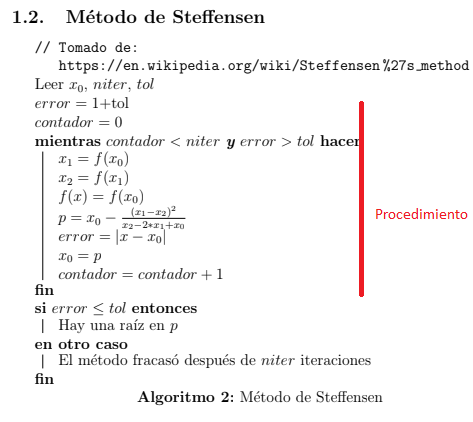
\includegraphics[height=230pt]{images/procedimiento.png}
	\end{frame}
	\begin{frame}{Procedimiento}
		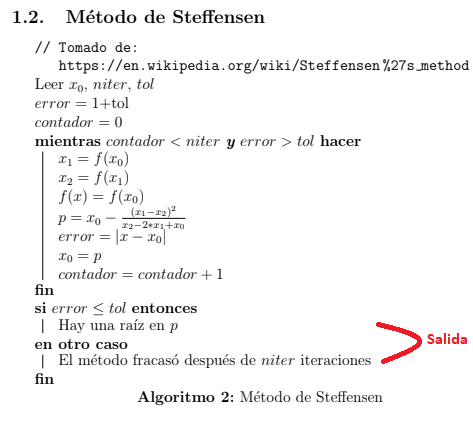
\includegraphics[height=230pt]{images/salida.png}
	\end{frame}
	\section{Octave}
	\subsection{Introducción}
	\begin{frame}{Introducción}
	\begin{itemize}[<+- | alert@ +>]
		\item Lenguaje de programación principalmente diseñado para trabajar con cálculos computacionales.
		\item Corre en distintas plataformas.
		\item Código interpretado.
	\end{itemize}
	\end{frame}
	\begin{frame}{Características}
	\begin{itemize}[<+- | alert@+>]
		\item Potente en cálculo computacional.
		\item Fácil de usar para este tipo de trabajos.
		\item Sintaxis clara.
		\item Lenguaje común entre los científicos de datos y personas que trabajan con cálculo computacional.
		\item Modularidad completa.
	\end{itemize}
	\end{frame}
	\begin{frame}{Primeros Pasos}
		\begin{itemize}
			\item [] \begin{block}{Hello Name!}
			\inputminted[xleftmargin=\parindent,linenos]{octave}{codes/hello.m}
		\end{block}
		\pause
		\item [] \begin{block}{Program 1}
			\inputminted[xleftmargin=\parindent,linenos]{python}{codes/program1.m}
			\end{block}
		\end{itemize}
	\end{frame}
	\begin{frame}{Primeros Pasos}
		\begin{itemize}
			\item []
			\begin{block}{Program 2}
				\inputminted[xleftmargin=\parindent,linenos]{python}{codes/program2.m}
			\end{block}
		\end{itemize}
	\end{frame}
	\begin{frame}{Primeros Pasos | Ejercicio}
			\begin{itemize}
				\item Lea dos enteros $x$, $y$ de la entrada estandar e imprima el valor de $x^y$ con una precisión de $5$ decimales correctos.
			\end{itemize}
		\end{frame}
	\subsection{Tipos de Datos I}
	\begin{frame}{Tipos de Datos I}
		\begin{itemize}[<+- | alert@ +>]
			\item Existen principalmente tres tipos de datos.
			\item Tipos Numéricos: \textbf{scalar, vector, matrix, complex.}
			\item Tipos Cadena: \textbf{Char}.
			\item Tipos Estructura de Datos. 
			\item Tipos definidos por el usuario.
		\end{itemize}
	\end{frame}
	\begin{frame}{Tipos de Datos I}
		\begin{block}{Program 3}
			\inputminted[xleftmargin=\parindent,linenos]{python}{codes/program3.m}
		\end{block}
	\end{frame}
	\subsection{Casting}
	\begin{frame}{Casting}
		\begin{itemize}
			\item Es el acto de pasar de un tipo de objeto a otro.
			\pause
			\item[] \begin{block}{Program 4}
				\inputminted[xleftmargin=\parindent,linenos]{python}{codes/program4.m}
			\end{block} 
		\end{itemize}
	\end{frame}
	\subsection{Documentación}
	\begin{frame}{Documentación}
		\begin{itemize}
			\item Se puede usar \textbf{help()} para obtener ayuda general en línea.
			\pause
			\item Usar \textbf{doc()} para una ayuda general más específica.
			\pause
			\item Usar \textbf{doc \textit{obj}} para saber información detallada de un tipo de dato u objeto.
			\pause
			\item [] 
			\begin{block}{Program 5}
				\inputminted[xleftmargin=\parindent,linenos]{python}{codes/program5.m}
			\end{block}
		\end{itemize}
	\end{frame}
	\subsection{Estructuras de Control}
	\begin{frame}{Estructuras de Control}
		\begin{itemize}[<+- | alert@ +>]{}
			\item Los programas se ejecutan de manera \textbf{secuencial}.
			\item A veces el desarrollador quiere que el programa no siga una secuencia específica sino que tome un \textit{camino} especifico.
			\item Las estructuras de control \textbf{if}, \textbf{for}, \textbf{while}, etc. nos permiten indicarle esos casos al código. 
		\end{itemize}
	\end{frame}
	\begin{frame}[allowframebreaks]{Instrucción \textbf{if}}
	\begin{itemize}
		\item [] \begin{block}{\textbf{if} Statement 1}
			\inputminted[xleftmargin=\parindent,linenos]{python}{codes/if_statement.m}
		\end{block}
		\pause
		\item [] \begin{block}{\textbf{if} Statement 2}
			\inputminted[xleftmargin=\parindent,linenos]{python}{codes/if_statement2.m}
		\end{block}
	\end{itemize}
	\end{frame}
	\begin{frame}{Operadores relacionales}
	\begin{itemize}
		\item \textbf{Comparación}: $==$, $<$, $>$, $<=$, $>=$, $!=$.
		\pause
		\item \textbf{And/Or}: \text{a $\&\&$ b}, \text{a 
			$\mid\mid$ b}.
		\pause
		\item \textbf{Not}: \textbf{not}
		\pause
		\item [] \begin{block}{Relationals}
			\inputminted[xleftmargin=\parindent,linenos]{python}{codes/relational.m}
		\end{block}
	\end{itemize}
	\end{frame}
	\begin{frame}{Operadores Relaciones | Ejercicio}
		\begin{itemize}
		\item Lea dos valores $x$, $y$ de la entrada estandar e imprima \textbf{YES} si existe algún valor $a$, tal qué $y = ax$. En caso contrario imprima \textbf{NO}.
		\end{itemize}
	\end{frame}
	\begin{frame}{Instrucción \textbf{while}}
	\begin{itemize}
		\item Esta instrucción ejecuta el contenido que está indentando hasta que la condición evaluada es falsa.
		\pause
		\item [] \begin{block}{\textbf{while} Statement}
			\inputminted[xleftmargin=\parindent,linenos]{python}{codes/while_statement.m}
		\end{block}
	\end{itemize}
	\end{frame}
	\begin{frame}{Instrucción \textbf{for}}
	\begin{itemize}
		\item Se usa principalmente para iterar sobre \textbf{rangos}.
		\pause
		\item Es muy útil en los casos donde yo conozco cual es l número de iteraciones fijas.
		\pause
		\item Es la herramienta principal para iterar sobre listas y otras estructuras de datos.
		\pause
		\item [] \begin{block}{\textbf{for} Statement}
			\inputminted[xleftmargin=\parindent,linenos]{python}{codes/for_statement.m}
		\end{block}
	\end{itemize}
	\end{frame}
	\begin{frame}[allowframebreaks]{Instrucción \textbf{for} continuación.}
	\begin{itemize}
	\item [] \begin{block}{\textbf{for} Statement 2}
		\inputminted[xleftmargin=\parindent,linenos]{python}{codes/for_statement2.m}
	\end{block}
		\begin{block}{\textbf{for} Statement 3}
		\inputminted[xleftmargin=\parindent,linenos]{python}{codes/for_statement3.m}
	\end{block}
	\end{itemize}
	\end{frame}
	\subsection{Funciones}
	\begin{frame}{Funciones}
		\begin{itemize}[<+- | alert@ +>]
			\item Cuando existen secuencias de código que se repiten varias veces dentro (del código), se pueden agrupar en funciones.
			\item Una función recibe cero o más parámetros de entrada y devuelve cero o más resultados.
			\item Los cálculos se realizan directamente dentro de la función.
			\item Las variables declaradas dentro de la función no son visibles a otras funciones.
			\item Son muy útiles para reutilizar código.
			\item ¡Se van a usar ampliamente en el curso!
		\end{itemize}
	\end{frame}
	\begin{frame}{Funciones | Declaración}
	\begin{itemize}
		\item \begin{block}{Functions}
			\inputminted[xleftmargin=\parindent,linenos]{python}{codes/decl_functions.m}
		\end{block}
	\end{itemize}
	\end{frame}
	\begin{frame}{Funciones | Declaración Continuación}
	\begin{itemize}
		\item [] \begin{block}{Functions 2}
			\inputminted[xleftmargin=\parindent,linenos]{python}{codes/decl_functions2.m}
		\end{block}
	\end{itemize}
	\end{frame}
	\begin{frame}{Funciones | Declaración Continuación}
	\begin{itemize}
		\item [] \begin{block}{Functions 3}
			\inputminted[xleftmargin=\parindent,linenos]{python}{codes/decl_functions3.m}
		\end{block}
	\end{itemize}
	\end{frame}
	\subsection{Entrada y Salida}
	\begin{frame}{Entrada y Salida}
		\begin{itemize}
			\item Todos los programas que construimos tiene salida y/o entrada.
			\pause
			\item [] \begin{block}{Input/Output}
				\inputminted[xleftmargin=\parindent,linenos]{python}{codes/input_output.m}
			\end{block}
		\end{itemize}
	\end{frame}
\section{Python (Opcional)}
\subsection{Introducción}
\begin{frame}{Introducción}
\begin{itemize}[<+- | alert@ +>]
	\item Lenguaje de programación dinámico que soporta diferentes paradigmas de programación.
	\item Código independiente de la plataforma.
	\item Código interpretado.
\end{itemize}
\end{frame}
\begin{frame}{Características}
\begin{itemize}[<+- | alert@+>]
\item Lenguaje extremadamente versátil.
\item Sintaxis clara.
\item Lenguaje común.
\item Modularidad completa.
\item Gran Comunidad.
\end{itemize}
\end{frame}
\begin{frame}{Primeros Pasos}
\begin{itemize}
\item [] \begin{block}{Hello Name!}
\inputminted[xleftmargin=\parindent,linenos]{octave}{codes/hello.py}
\end{block}
\pause
\item [] \begin{block}{Program 1}
\inputminted[xleftmargin=\parindent,linenos]{python}{codes/program1.py}
\end{block}
\end{itemize}
\end{frame}
\begin{frame}{Primeros Pasos}
\begin{itemize}
\item []
\begin{block}{Program 2}
\inputminted[xleftmargin=\parindent,linenos]{python}{codes/program2.py}
\end{block}
\end{itemize}
\end{frame}
	\subsection{Tipos de Datos I}
	\begin{frame}{Tipos de Datos I}
		\begin{itemize}[<+- | alert@ +>]
			\item Los \textbf{objetos} son el núcleo de las cosas que Python puede manipular.
			\item Cada objeto tiene un tipo.
			\item Los tipos son \textbf{escalares} o \textbf{no-escalares}.
			\item Los tipos escalares son: \textbf{int}, \textbf{float}, \textbf{bool} y \textbf{None}.
			\item Los objetos y los \textbf{operadores} pueden usarse para formar \textbf{expresiones}.
		\end{itemize}
	\end{frame}
	\begin{frame}{Tipos de Datos I}
		\begin{block}{Program 3}
			\inputminted[xleftmargin=\parindent,linenos]{python}{codes/program3.py}
		\end{block}
	\end{frame}
	\subsection{Casting}
	\begin{frame}{Casting}
		\begin{block}{Program 4}
			\inputminted[xleftmargin=\parindent,linenos]{python}{codes/program4.py}
		\end{block}
	\end{frame}
	\subsection{Documentación}
		\begin{frame}{Documentación}
			\begin{itemize}
				\item Se puede usar \textbf{help()} para obtener ayuda general en línea.
				\pause
				\item Se puede usar \textbf{help(\textit{obj})} para consultar sobre un objeto específico.
				\pause
				\item Usar \textbf{dir()} para saber todos los nombres usados.
				\pause
				\item Usar \textbf{dir(\textit{obj})} para saber todos los nombres usados por un objeto.
				\pause
				\item [] 
				\begin{block}{Program 5}
					\inputminted[xleftmargin=\parindent,linenos]{python}{codes/program5.py}
				\end{block}
			\end{itemize}
		\end{frame}
\subsection{Estructuras de Control}
\begin{frame}[allowframebreaks]{Instrucción \textbf{if}}
	\begin{itemize}
		\item [] \begin{block}{\textbf{if} Statement 1}
			\inputminted[xleftmargin=\parindent,linenos]{python}{codes/if_statement.py}
		\end{block}
		\pause
		\item [] \begin{block}{\textbf{if} Statement 2}
			\inputminted[xleftmargin=\parindent,linenos]{python}{codes/if_statement2.py}
		\end{block}
	\end{itemize}
	\end{frame}
	\begin{frame}{Operadores relacionales}
		\begin{itemize}
			\item \textbf{Comparación}: $==$, $<$, $>$, $<=$, $>=$, $!=$.
			\pause
			\item \textbf{Comparación de objetos}: \text{a \textbf{is} b}, 
			\text{a \textbf{is not} b}.
			\pause
			\item \textbf{And/Or}: \text{a \textbf{and} b}, \text{a 
				\textbf{or} b}.
			\pause
			\item \textbf{Not}: \textbf{not}
			\pause
			\item [] \begin{block}{Relationals}
				\inputminted[xleftmargin=\parindent,linenos]{python}{codes/relational.py}
			\end{block}
		\end{itemize}
	\end{frame}
	\begin{frame}{Instrucción \textbf{while}}
		\begin{block}{\textbf{while} Statement}
			\inputminted[xleftmargin=\parindent,linenos]{python}{codes/while_statement.py}
		\end{block}
	\end{frame}
	\begin{frame}{Instrucción \textbf{for}}
		\begin{block}{\textbf{for} Statement}
			\inputminted[xleftmargin=\parindent,linenos]{python}{codes/for_statement.py}
		\end{block}
	\end{frame}
	\begin{frame}[allowframebreaks]{Instrucción \textbf{for} continuación.}
		\begin{itemize}
		\item [] \begin{block}{\textbf{for} Statement 2}
			\inputminted[xleftmargin=\parindent,linenos]{python}{codes/for_statement2.py}
		\end{block}
			\begin{block}{\textbf{for} Statement 3}
			\inputminted[xleftmargin=\parindent,linenos]{python}{codes/for_statement3.py}
		\end{block}
		\end{itemize}
	\end{frame}
\subsection{Funciones}
	\begin{frame}{Funciones | Declaración}
	\begin{itemize}
		\item \begin{block}{Functions}
			\inputminted[xleftmargin=\parindent,linenos]{python}{codes/decl_functions.py}
		\end{block}
	\end{itemize}
	\end{frame}
	\begin{frame}{Funciones | Declaración Continuación}
	\begin{itemize}
		\item [] \begin{block}{Functions 2}
			\inputminted[xleftmargin=\parindent,linenos]{python}{codes/decl_functions2.py}
		\end{block}
	\end{itemize}
	\end{frame}
	\begin{frame}{Funciones | Declaración Continuación}
	\begin{itemize}
		\item [] \begin{block}{Functions 3}
			\inputminted[xleftmargin=\parindent,linenos]{python}{codes/decl_functions3.py}
		\end{block}
	\end{itemize}
	\end{frame}
	\subsection{Entrada y Salida}
	
	\subsection{Errores y Excepciones}
		\begin{frame}{Errores y Excepciones}
		\begin{itemize}[<+- | alert@ +>]
			\item Cuando nuestro código se está ejecutando, pueden surgir errores durante la ejecución.
			\item División por cero.
			\item Leer un archivo que no existe.
			\item Escribir en un archivo de solo lectura.
			\item $\cdots$.
		\end{itemize}
		\end{frame}
		\begin{frame}{Errores y Excepciones Continuación}
		\begin{block}{Input/Output}
			\inputminted[xleftmargin=\parindent,linenos]{python}{codes/exceptions.py}
		\end{block}
		\end{frame}
		\subsection{Tipos de Datos II}
		\begin{frame}{Tipos de Datos II}
			\begin{itemize}[<+- | alert@ +>]
				\item \textbf{[]}. Lista de elementos.
				\item \textbf{List}: Estructura ordenada, admite elementos repetidos. 
				\item \textbf{Set}: Estructura no ordenada, no hay elementos duplicados.
				\item \textbf{Dictionary}: Estructura no ordenada, la forma de acceder y escribir es \textit{clave, valor}. $f(x) = y$.
			\end{itemize}
		\end{frame}
		\begin{frame}{Tipos de Datos II Continuación}
			\begin{block}{Structures}
				\inputminted[xleftmargin=\parindent,linenos]{python}{codes/structures.py}
			\end{block}
		\end{frame}
		\subsection{Módulos y Paquetes}
		\begin{frame}{Módulos y Paquetes}
			\begin{block}{Modules}
				\inputminted[xleftmargin=\parindent,linenos]{python}{codes/modules.py}
			\end{block}
		\end{frame}
		\subsection{Técnicas Avanzadas}
		\begin{frame}{Técnicas Avanzadas}
		\begin{itemize}[<+- | alert@ +>]
			\item \textbf{Sliding}
			\item \textbf{Condicionales}
			\item \textbf{Agrupación}
			\item \textbf{Listas}
			\item \textbf{Simplificación}
		\end{itemize}
		\end{frame}
		\begin{frame}{Técnicas Avanzadas Continuación}
			\begin{block}{Advanced}
				\inputminted[xleftmargin=\parindent,linenos]{python}{codes/advanced_techniques.py}
			\end{block}
		\end{frame}
		\subsection{Computación Numérica}
		\begin{frame}{Computación Numérica}
			\begin{itemize}[<+- | alert@ +>]
				\item Cálculos lineales y no lineales.
				\item Operaciones matriciales.
				\item Precisión Numérica.
				\item Simplificación dirigida.
				\item Optimización.
				\item \textbf{numpy}
				\item $\cdots$
			\end{itemize}
		\end{frame}
		\begin{frame}{Computación Numérica Continuación}
			\begin{block}{Numeric}
				\inputminted[xleftmargin=\parindent,linenos]{python}{codes/numerical_computation.py}
			\end{block}
		\end{frame}
		\subsection{Cálculo Simbólico}
		\begin{frame}{Cálculo Simbólico}
		\begin{itemize}[<+- | alert@ +>]
			\item Diferenciación.
			\item Integración.
			\item Simplificación.
			\item Correlación.
			\item Evaluación.
			\item \textbf{sympy}
			\item $\cdots$
		\end{itemize}
		\end{frame}
		\begin{frame}{Computación Simbólica Continuación}
		\begin{block}{Symbolic}
		\inputminted[xleftmargin=\parindent,linenos]{python}{codes/symbolic_computation.py}
		\end{block}
		\end{frame}
		\subsection{Gráficos}
		\begin{frame}{Gráficos}
		\begin{itemize}[<+- | alert@ +>]
			\item 1D
			\item 2D
			\item 3D
			\item Intersección.
			\item Aproximación.
			\item \textbf{matplotlib}.
			\item $\cdots$
		\end{itemize}
	\end{frame}
	\begin{frame}{Gráficos Continuación}
	\begin{block}{Graphs}
	\inputminted[xleftmargin=\parindent,linenos]{python}{codes/graphs.py}
	\end{block}
	\end{frame}
	\begin{frame}[standout]
	Gracias!
	\end{frame}
\end{document}